%% logues.tex
%% Author: Leighton Pritchard
%% Copyright: James Hutton Institute
%% Who let the -logues out?

%
\begin{frame}
  \frametitle{Who let the -logues out?}
  \Large{
    \textcolor{olive}{
      \textbf{
      Genome features can have complex evolutionary relationships \\~\\
      We need precise terms to describe these relationships
      }
    }
  }
  \begin{center}
    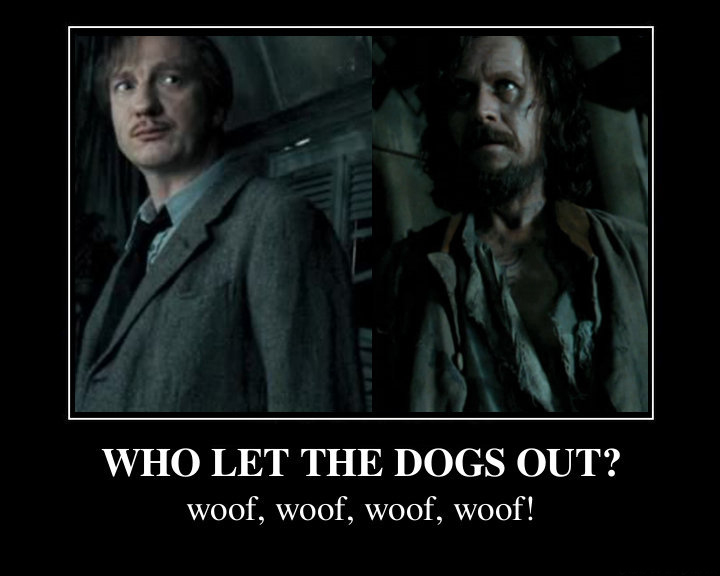
\includegraphics[width=0.4\textwidth]{images/who_let_the_dogs_out}
  \end{center}      
\end{frame}

%
\begin{frame}
  \frametitle{The -logues drop
  \footnote{\tiny{\href{http://dx.doi.org/10.2307/2412448
}{Fitch \textit{et al.} (1970) \textit{Syst. Zool.} doi:10.2307/2412448
}}}
  }
  How do we understand the relationships between features in more than one genome?
  \begin{itemize}
    \item \textcolor{hutton_green}{Functional similarity}: \textbf{analogy}
    \item \textcolor{hutton_blue}{Evolutionary common origin}: \textbf{homology, orthology, etc.}
    \item \textcolor{hutton_purple}{Evolutionary/functional/family relationship}: \textbf{paralogy}
  \end{itemize}
  \begin{center}
    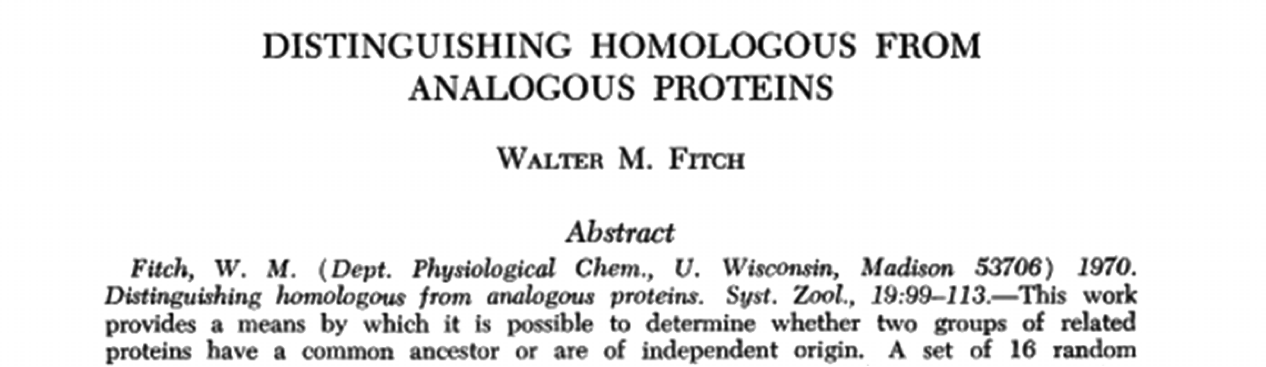
\includegraphics[width=\textwidth]{images/fitch}
  \end{center}    
\end{frame}

%
\begin{frame}
  \frametitle{Definitions
  }
  Technical terms describing evolutionary relationships
  \begin{itemize}
    \item \textbf{\textcolor{hutton_blue}{Homologues}}: share a common ancestor \textcolor{red}{\textbf{NOTE: there are NOT degrees of homology}}
    \item \textbf{\textcolor{hutton_blue}{Analogues}}: are functionally similar. Analogues may or may not share common ancestry
    \item \textbf{\textcolor{hutton_green}{Orthologues}}: are homologues that \textit{diverged through speciation}
    \item \textbf{\textcolor{hutton_purple}{Paralogues}}: are homologues that \textit{diverged through duplication} within the same genome
  \end{itemize}
  (also \textit{co-orthologues}, \textit{xenologues}, etc.)
\end{frame}